% This text is proprietary.
% It's a part of presentation made by myself.
% It may not used commercial.
% The noncommercial use such as private and study is free
% Nov. 2006
% Author: Sascha Frank 
% University Freiburg 
% www.informatik.uni-freiburg.de/~frank/
%
% additional usepackage{beamerthemeshadow} is used
%  
%  \beamersetuncovermixins{\opaqueness<1>{25}}{\opaqueness<2->{15}}
%  with this the elements which were coming soon were only hinted
\documentclass{beamer}
\usepackage{beamerthemeshadow}
\usepackage{verbatim}
\usepackage{lipsum}
\usepackage{xcolor}

\newcommand\Fontvismall{\fontsize{5}{4}\selectfont}
\newcommand\Fontvi{\fontsize{9}{7.2}\selectfont}
\newcommand\Fontvilarge{\fontsize{10}{8}\selectfont}
\setbeamerfont{footline}{size=\fontsize{9}{11}\selectfont \title{The ReqWiki Approach \hspace{3em} \insertframenumber/\inserttotalframenumber}}

\begin{document}

\AtBeginSection[]
{
  \begin{frame}
    \frametitle{Table of Contents}
    \tableofcontents[currentsection]
  \end{frame}
}

\titlegraphic{
\includegraphics[width=.15\textwidth,height=.15\textheight]{MST}}
\title{ReqWiki: A Semantic System for Collaborative Software Requirements Engineering with Integrated Text Analysis Support}  
\author{Anurag Panwar}
\institute{Department of Computer Science\\
Missouri University of Science and Technology}
\date{December 1,2014} 

\frame{\titlepage} 

\begin{comment}
\frame{\frametitle{Table of contents}\tableofcontents} 
\end{comment}

\section{Introduction} 
\subsection{Motivation}
\frame{\frametitle{Motivation} 
\begin{itemize}
\Fontvi
\item Requirements Engineering (RE) is the process of eliciting, evaluating, and recording the needs of various stakeholders of a software project
\item Heavily knowledge-driven and collaborative task
\item Critical to building "the right product"
\begin{figure}
   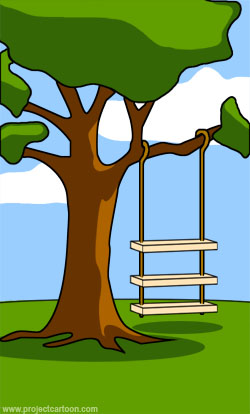
\includegraphics[width=0.2\textwidth]{1}
   \hfill
   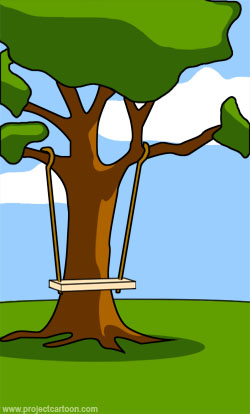
\includegraphics[width=0.2\textwidth]{2}
   \hfill
   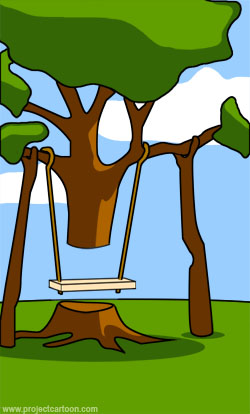
\includegraphics[width=0.2\textwidth]{3}
   \hfill   
   
\includegraphics[width=0.2\textwidth]{4}
\end{figure}
\end{itemize}
}

\subsection{Introduction}
\frame{\frametitle{Introduction}
\Fontvi
\begin{block}{Software Requirements Specifcations (SRS)}
\begin{itemize}
\Fontvi
\item Up to 90 of requirements specifications are written in natural language 
\item Inherent ambiguity in using natural language
\item Support Unified Process (UP) methodology
\item Use Cases, Test Cases, etc.
\end{itemize}
\end{block}


\begin{exampleblock}{SRS Tools}
\begin{itemize}
\item Enterprise tools vs. general Office tools (used in SMEs)
\item Wikis recently emerged as affordable collaborative tools in RE
\item Wikis require structure and customization for RE
\end{itemize}
\end{exampleblock} 


\begin{alertblock}{Intelligent Assistants}
\begin{itemize}
\item Automated "assistants" that work collaboratively with humans on SRS
\item Using Natural Language Processing (NLP) for quality assurance
\item Semantic technologies (ontologies) for traceability, etc.
\end{itemize}
\end{alertblock}
}

\subsection{Natural Language Processing (NLP)}
\frame{\frametitle{Natural Language Processing (NLP)}
\begin{itemize}
\item A branch of Artificial Intelligence
\begin{itemize}
\Fontvi
\item uses various techniques to process content written in natural language
\end{itemize}
\item Multitude of NLP techniques
\begin{itemize}
\Fontvi
\item Named Entity Recognition (e.g., Finding Persons, Organizations, etc.)
\item Quality Assessment
\item Summarization
\end{itemize}
\item Various NLP APIs (e.g., OpenCalais, GATE, . . . )
\end{itemize}
\begin{figure}
 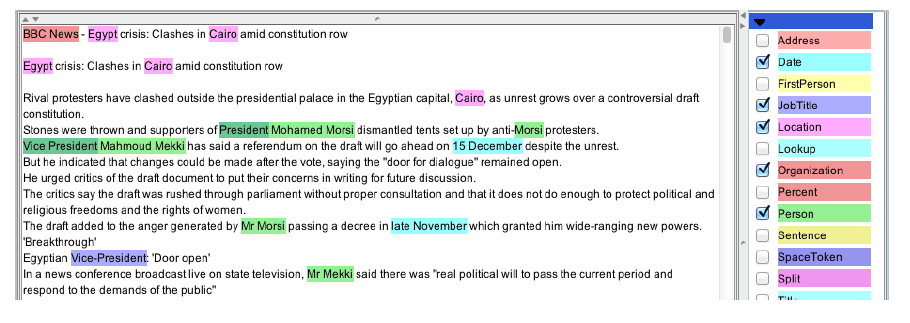
\includegraphics[width=0.8\textwidth]{NLP_intro}
\end{figure}
}

\subsection{Semantic Assistants}
\frame{\frametitle{Semantic Assistants}
\begin{itemize}
\item Service-oriented Architecture (SOA)
\item Publishes various NLP pipelines as W3C Standard Web services
\item Open source framework (http://www.semanticassistants.com)
\end{itemize}
\begin{figure}
 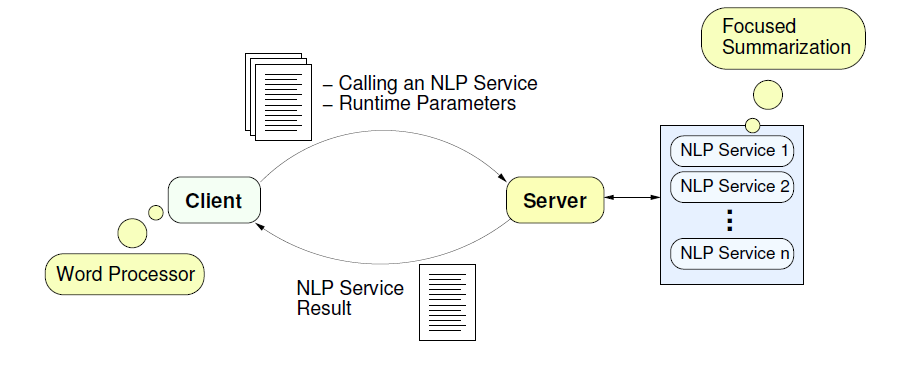
\includegraphics[width=1\textwidth]{semantic_assistants}
\end{figure}
}

\begin{comment}
\begin{alertblock}{Challenges}
The proposed system must
\begin{enumerate}
\item Support arbitrary standard software engineering methodologies
\item Not require prior background knowledge in NLP or Semantic technologies
\end{enumerate}
\end{alertblock} 
\end{comment}


\section{The ReqWiki Approach} 
\subsection{ReqWiki Architecture}
\frame{\frametitle{ReqWiki Architecture}
\begin{itemize}
\item Collaborative RE platform with integrated text analysis support 
\item Powered by the MediaWiki engine
\item Based on the Semantic Assistants Wiki-NLP Integration
\item Provides seamless integration of NLP capabilities within wikis
\item Includes ontological formalization of SRS entities and their relationships
\end{itemize} 
\begin{figure}
 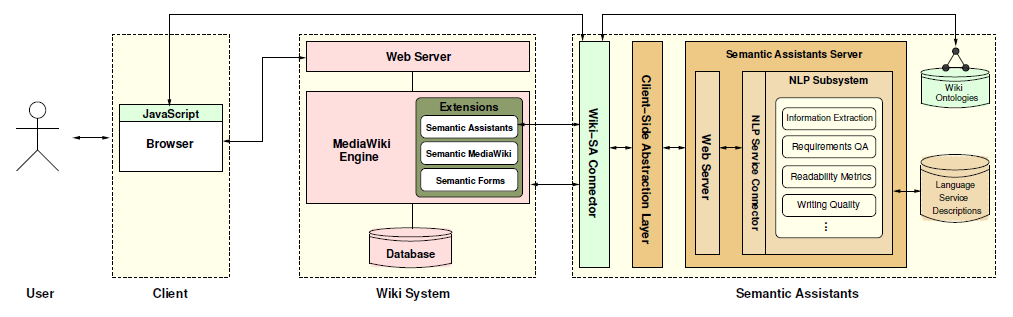
\includegraphics[width=1\textwidth]{reqwiki_archi}
\end{figure}
}

\subsection{Semantic model for SRS}
\frame{\frametitle{Semantic model for SRS}
\begin{itemize}
\item Formally describe software artifacts and their components
\item Used to model, connect and query SRS statements with ontology concepts
\end{itemize} 
\begin{figure}
 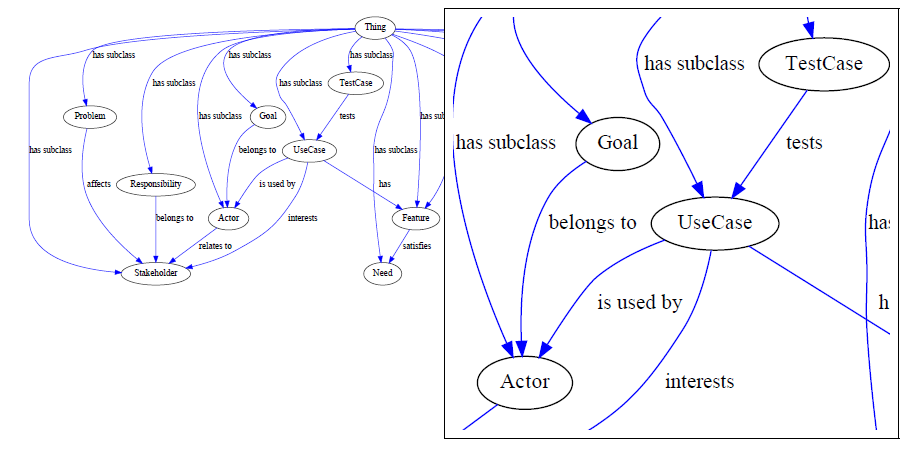
\includegraphics[width=1\textwidth]{semantic}
\end{figure}
}

\subsection{User Interface}
\frame{\frametitle{User Interface}
\Fontvi
\begin{itemize}
\item Semantic MediaWiki customized for collaborative requirements engineering
\item Follows Unified Process (UP) methodology
\item Structures SRS artifacts using forms and templates based on ontology
\end{itemize} 
\begin{figure}
 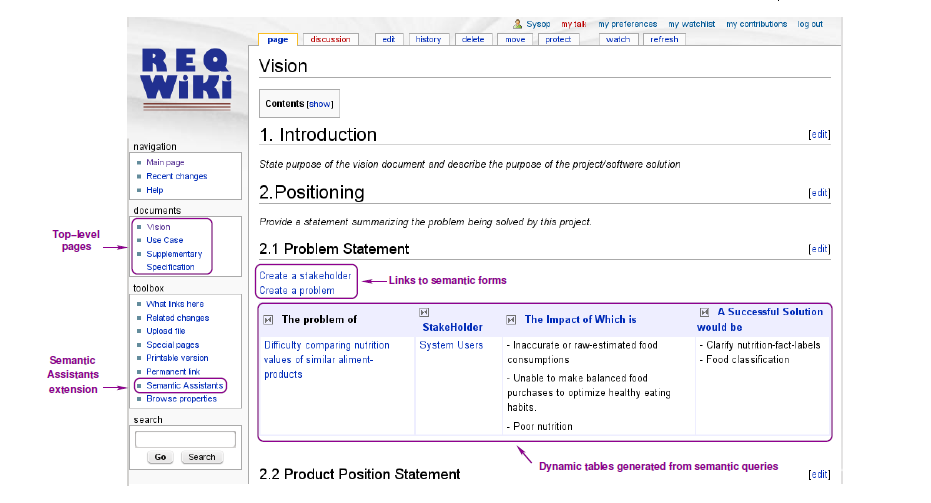
\includegraphics[width=0.9\textwidth]{UI}
\end{figure}
}

\subsection{Features}
\frame{\frametitle{Semantic forms}
\begin{itemize}
\item Semantic Forms as data entry point
\item Structures content at fner granularities
\item Automatically generates RDF markup for linking and querying
\end{itemize} 
\begin{figure}
 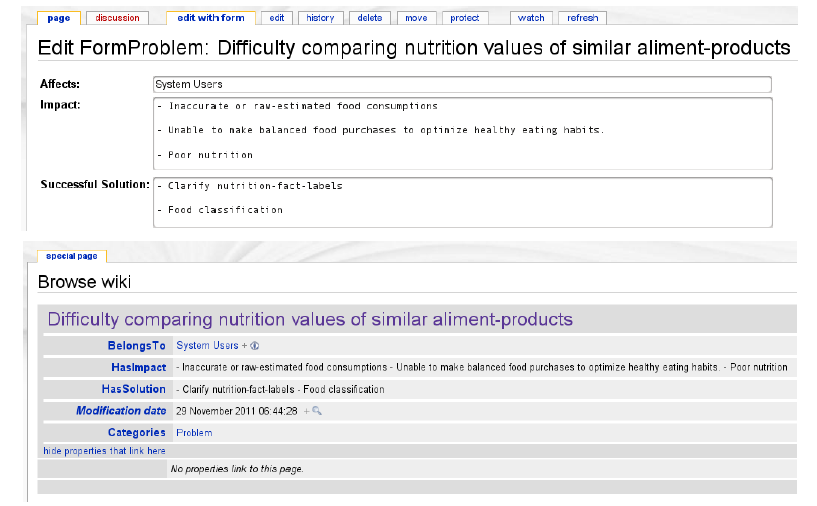
\includegraphics[width=0.9\textwidth]{semantic_form}
\end{figure}
}

\frame{\frametitle{Automatic Traceability}
\Fontvilarge
\begin{itemize}
\item Traceability is concerned with interrelating various software artifacts
\item Manually cross-referencing documents is time-consuming and error-prones
\item Leverage the semantic metadata in ReqWiki
\item Traceability Links
\begin{enumerate}
\Fontvilarge
\item Revision links
\item Semantic links
\item Query-based links
\end{enumerate}
\end{itemize} 
\begin{figure}
 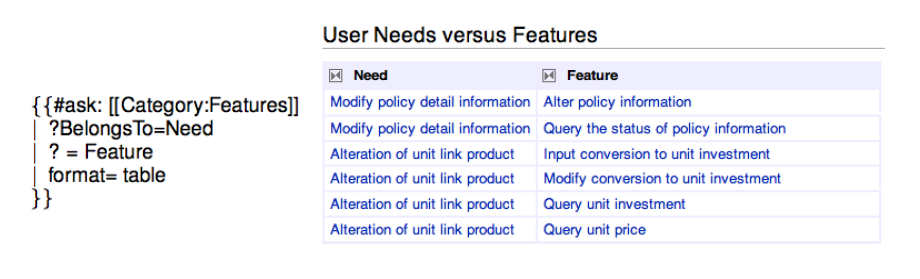
\includegraphics[width=0.9\textwidth]{traceability}
\end{figure}
}

\frame{\frametitle{ReqWiki NLP services}
\Fontvi
\begin{columns}[T] % align columns
\begin{column}{.50\textwidth}
\begin{itemize}
\item Various NLP services
\begin{figure}
 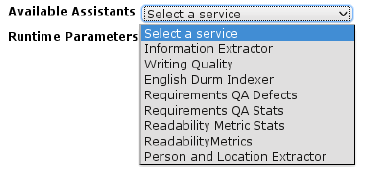
\includegraphics[width=0.8\textwidth]{NLP}
\end{figure}
\item SRS defects addressable
\begin{itemize}
\Fontvi
\item Spelling and Grammar
\item Incompleteness
\item Ambiguity
\item Poor Structuring
\item Passive voice
\item etc
\end{itemize}

\item Automatically index the SRS
\begin{itemize}
\Fontvi
\item back-of-the-book style
\item complement the glossary
\item helping domain analysis
\end{itemize}

\end{itemize}


\end{column}%
\hfill%
\begin{column}{.50\textwidth}
\begin{figure}
 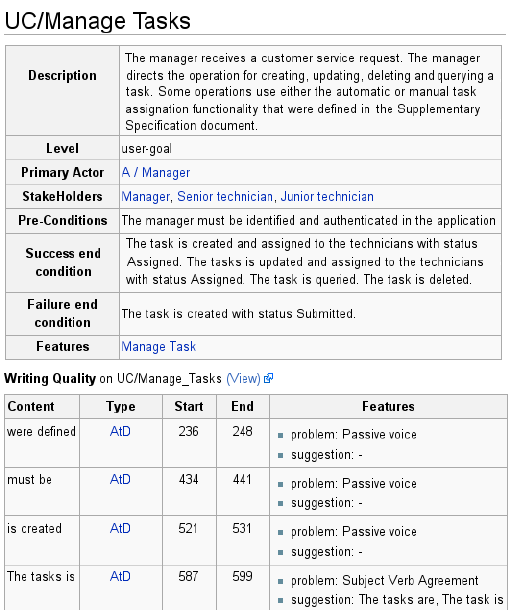
\includegraphics[width=1\textwidth]{NLP_services}
\end{figure}
\end{column}%
\end{columns}
}



\section{Evaluation} 
\subsection{Effectiveness}
\frame{\frametitle{User Study I - Effectiveness}
\begin{itemize}
\Fontvi
\item Can text mining assistants help to improve requirements specifications?
\item User study with 2 software engineering classes
\begin{itemize}
\Fontvi
\item \textcolor{blue}{Goal:} Identifying defects in manual vs. NLP-assisted requirements specifications
\item \textcolor{blue}{NLP Services:}Spell checking, Readability Analysis, Passive Voice Detection,...
\item \textcolor{blue}{Measure:} Average number of defects found in the two assignment revisions
\item \textcolor{blue}{Method:} Comparison of manual vs. NLP-assisted quality assurance
\end{itemize}
\end{itemize}
\begin{figure}
 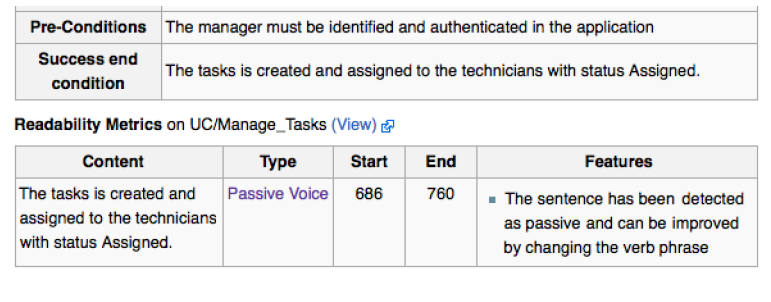
\includegraphics[width=1\textwidth]{example}
\end{figure}
}

\frame{\frametitle{User Study I - Effectiveness}
User study Results
\begin{figure}
 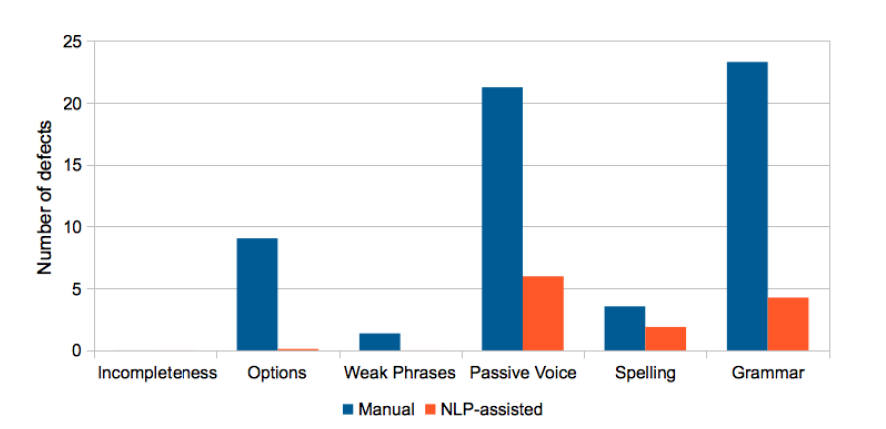
\includegraphics[width=0.8\textwidth]{result}
\end{figure}
\begin{exampleblock}{Conclusion}
ReqWiki NLP capabilities were indeed effective to significantly reduce SRS
defects.
\end{exampleblock} 
}

\subsection{Usability}
\frame{\frametitle{User Study 2 - Usability}
\begin{itemize}
\item User Study II - Usability
How much NLP background do users need in order to use semantic capabilities?
\item Same scenario as User Study I
\item Anonymized questionnaire asking participants about
\begin{enumerate}
\item Their proficiency level in NLP
\item ReqWiki ease-of-use
\end{enumerate}
\end{itemize}
\begin{figure}
 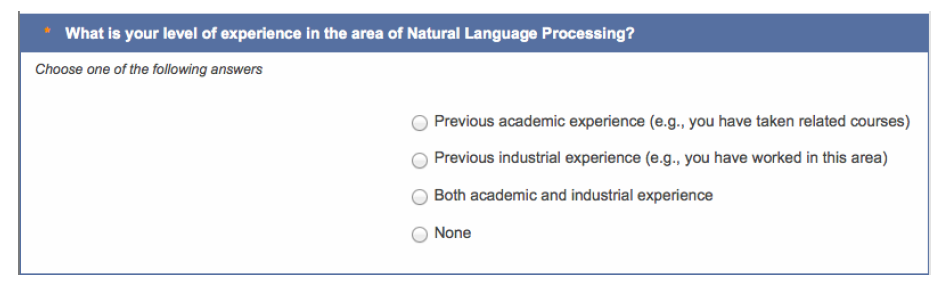
\includegraphics[width=0.8\textwidth]{usability}
\end{figure}
}

\frame{\frametitle{User Study 1 - Effectiveness}
User study Results
\begin{figure}
 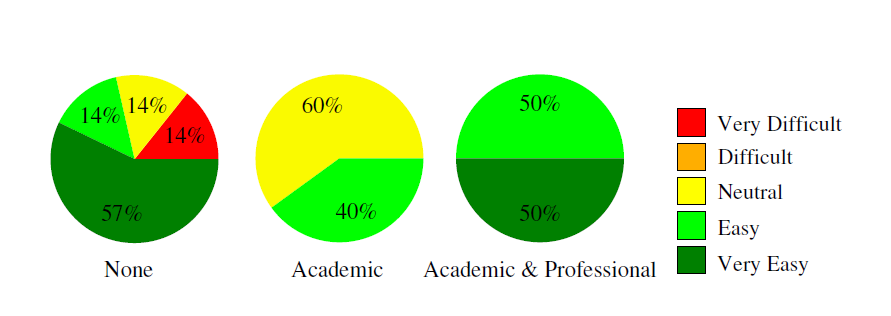
\includegraphics[width=1\textwidth]{study_result}
\end{figure}
\begin{exampleblock}{Conclusion}
Concrete NLP background is not required to make use of sophisticated
semantic support provided in ReqWiki.
\end{exampleblock} 
} 



\section{Conclusion}
\subsection{Summary and Outlook}
\frame{\frametitle{Summary and Outlook}
\begin{itemize}
\item ReqWiki is a semantic, collaborative platform for RE
\item Combination of modern semantic techniques can improve RE
\item Help in automate the Software requirements verification
\item Uses NLP techniques to find the ambiguous, incomplete, conflicting requirements
\item Saves a lot of time 
\end{itemize}


}


\end{document}
